\section{Проектирование программного обеспечения}

Вариантом реализации архитектуры может быть монолитное приложение, когда вся или большая часть бизнес-задач имеет одну кодовую базу.
Актуальным решением в настоящее время является построенное на микросервисах приложение, в котором общая бизнес-задача разбита на отдельные части, каждая из которых имеет отдельное приложение (микросервис) со своей кодовой базой[13].
\bigbreak
Монолитное приложение(далее монолит) представляет собой приложение, доставляемое через единое развертывание.
Таким является приложение, доставленное в виде одной WAR или приложение Node с одной точкой входа.

Достоинства:
\begin{itemize}
    \item Большим преимуществом монолита является то, что его легче реализовать;
    В монолитной архитектуре можно быстро начать реализовывать свою бизнес-логику, вместо того чтобы тратить время на размышления о межпроцессном взаимодействие;
    \item Сквозные (E2E) тесты. В монолитной архитектуре их легче выполнить;
    \item Говоря об операциях, важно сказать, что монолит прост в развертывании и легко масштабируется.
    Для развертывания можно использовать скрипт, загружающий ваш модуль и запускающий приложение. Масштабирование достигается путем размещения Loadbalancer перед несколькими экземплярами вашего приложения.
\end{itemize}
Недостатки:
\begin{itemize}
    \item Монолиты, как правило, перерождаются из своего чистого состояния в так называемый «большой шарик грязи».
    Вкратце это описывается как состояние, возникшее, потому что архитектурные правила были нарушены и со временем компоненты срослись.
    Это перерождение замедляет процесс разработки: каждую будущую функцию будет сложнее развивать.
    Из-за того что компоненты растут вместе, их также необходимо менять вместе.
    Создание новой функции может означать прикосновение к 5 различным местам: 5 мест, в которых нужно написать тесты; 5 мест, которые могут иметь нежелательные побочные эффекты для существующих функций;
    \item Выше оговаривалось, что в монолите легко масштабировать.
    Это действительно так до тех пор, пока он не перерастет в «большой шарик грязи», как упоминалось ранее.
    Масштабирование может быть проблематичным, когда только одной части системы требуются дополнительные ресурсы, ведь в монолитной архитектуре вы не можете масштабировать отдельные части вашей системы;
    \item В монолите практически нет изоляции.
    Проблема или ошибка в модуле может замедлить или разрушить все приложение;
    \item Строительство монолита часто протекает с помощью выбора основы.
    Отключение или обновление вашего первоначального выбора может быть затруднительным, потому что это должно быть сделано сразу и для всех частей вашей системы.
\end{itemize}
\bigbreak

В микросервисной архитектуре слабо связанные сервисы взаимодействуют друг с другом для выполнения задач, относящихся к их бизнес"=возможностям.

Микросервисы в значительной степени получили свое название из-за того, что сервисы здесь меньше, чем в монолитной среде. Тем не менее, микро — о бизнес-возможностях, а не о размере.

По сравнению с монолитом в микросервисах у имеется несколько единиц развертывания. Каждый сервис развертывается самостоятельно.

Достоинства:
\begin{itemize}
    \item Микросервисы легче держать модульными. Технически это обеспечивается жесткими границами между отдельными сервисами;
    \item В больших компаниях разные сервисы могут принадлежать разным командам.
    Услуги могут быть повторно использованы всей компанией.
    Это также позволяет командам работать над услугами в основном самостоятельно.
    Нет необходимости координировать развертывание между командами.
    Развивать весы лучше с увеличением количества команд;
    \item Микросервисы меньше, и благодаря этому их легче понять и проверить.
    Меньшие размеры помогают, когда речь идет о времени компиляции, времени запуска и времени, необходимом для выполнения тестов.
    Все эти факторы влияют на производительность разработчика, так как позволяют затрачивать меньше времени на ожидание на каждом этапе разработки;
    \item Более короткое время запуска и возможность развертывания микросервисов независимо друг от друга действительно выгодны для CI / CD.
    По сравнению с обычным монолитом он намного плавнее;
    \item Микросервисы не привязаны к технологии, используемой в других сервисах.
    Значит мы можем использовать лучшие технологии подгонки.
    Старые сервисы могут быть быстро переписаны для использования новых технологий;
    \item В микросервисах изолируемые разломы лучше по сравнению с монолитным подходом.
    Хорошо спроектированная распределенная система переживет сбой одного сервиса.
\end{itemize}

Недостатки:
\begin{itemize}
    \item Распределенная система имеет свою сложность: в ней приходится иметь дело с частичным отказом, более затруднительным взаимодействием при тестировании (тесты E2E), а также с более высокой сложностью при реализации взаимодействия между сервисами;
    \item Транзакции легче проводить в монолите.
    Решением этой проблемы на микросервисах является Saga Pattern.
    Хорошее решение, но все же слишком громоздкое для реализации на практике;
    \item Существуют эксплуатационные накладные расходы, а множество микросервисов сложнее в эксплуатации, чем несколько экземпляров сигнального монолита;
    \item Помимо вышеперечисленных сложностей, для микросервисов также может потребоваться больше оборудования, чем для традиционных монолитов.
    Иногда микросервисы могут превзойти один монолит, если есть его части, которые требуют масштабирования до предела;
    \item Изменения, затрагивающие несколько сервисов, должны координироваться между несколькими командами, а это может быть сложно, если команды еще не имели контактов.


\end{itemize}
\bigbreak

Так как дипломный проект представляет из себя хоть и законченный проект, но в то же время прототип, то было решено использовать монолитную архитектуру реализации проекта.
Несмотря на это, по причине того, что серверная часть написана на Django, который под собой разбивает приложение на набор небольших приложения, проблем с масштабированием данного приложения на сервисную архитектуру не должен составить труда.


\subsection{Проектирование базы данных БД}

\subsubsection{}

Первостепенной моделью данного проекта является пользователь, который при регистрации указывает свои контактные данные и краткую информацию о себе.

При регистрации пользователь выбирает себе аватар.

Пользователь может создать товар, заполнив некоторый набор полей о товаре.

При создании товара пользователь может добавлять некоторое количество фотографий товара и определять его в некоторые категории.

Пользователь может положить товар к себе в корзину.

Пользователь может купить товар в аренду либо сдать его.

Пользователь может сохранить методы оплаты.

Пользователь может сохранить адрес доставки товара.

Пользователь может оставлять отзывы о других пользователях.

Таким образом можно выделить сущности:
\begin{itemize}
    \item User – сущность, представляющая пользователя;
    \item Good - сущность, представляющая товар в системе;
    \item UserAvatar – сущность, предстваляющая аватар пользователя;
    \item GoodAvatar - сущность, представляющая фотографию товара;
    \item Tag - сущность, представляющая категории товара;
    \item Basket - сущность, предстввляющая корзину товаров пользователя;
    \item Payment - сущность, представляющая метод оплаты пользователя;
    \item Address - сущность, представляющая адрес доставки пользователя;
    \item Review - сущность, представляющая отзыв пользователя о пользователе;
    \item Order - сущность, представляющая товар, взятый в аренду пользователем;
    \item BasketGood - сущность, предствляющая товар, лежащий в корзине пользовтаеля.
\end{itemize}

Выделив сущности, можно составить связи между ними в таблице \ref{opisanie:suw}.


\begin{longtable}{ | l | l | l | }
    \caption{Описание связей сущностей}
    \label{opisanie:suw}
    \endfirsthead
    \endhead
    \hline
    Родительская сущность & Дочерняя сущность & Тип связи  \\ \hline
    User & UserAvatar & один-к-одному \\ \hline
    User & Basket & один-к-одному \\ \hline
    User & Good & один-ко-многим \\ \hline
    Good & GoodsAvatar & один-ко-многим \\ \hline
    Good & Tag & многие-ко-многим \\ \hline
    User & Payment & один-ко-многим \\ \hline
    User & Address & один-ко-многим \\ \hline
    User & Order & один-ко-многим \\ \hline
    User & Review & многие-ко-многим \\ \hline
    Basket & Good & многие-ко-многим \\ \hline
    Order & Good & многие-ко-многим  \\ \hline
    Payment & Order & один-ко-многим \\ \hline
    Address & Order & один-ко-многим \\
    \hline
\end{longtable}

\subsubsection{}

На основании выделенных сущностей и связей была составлина ER-диаграмма сущностей(см. рисунок \ref{db:erdiag}).

\begin{figure}[!h]
    \centering
    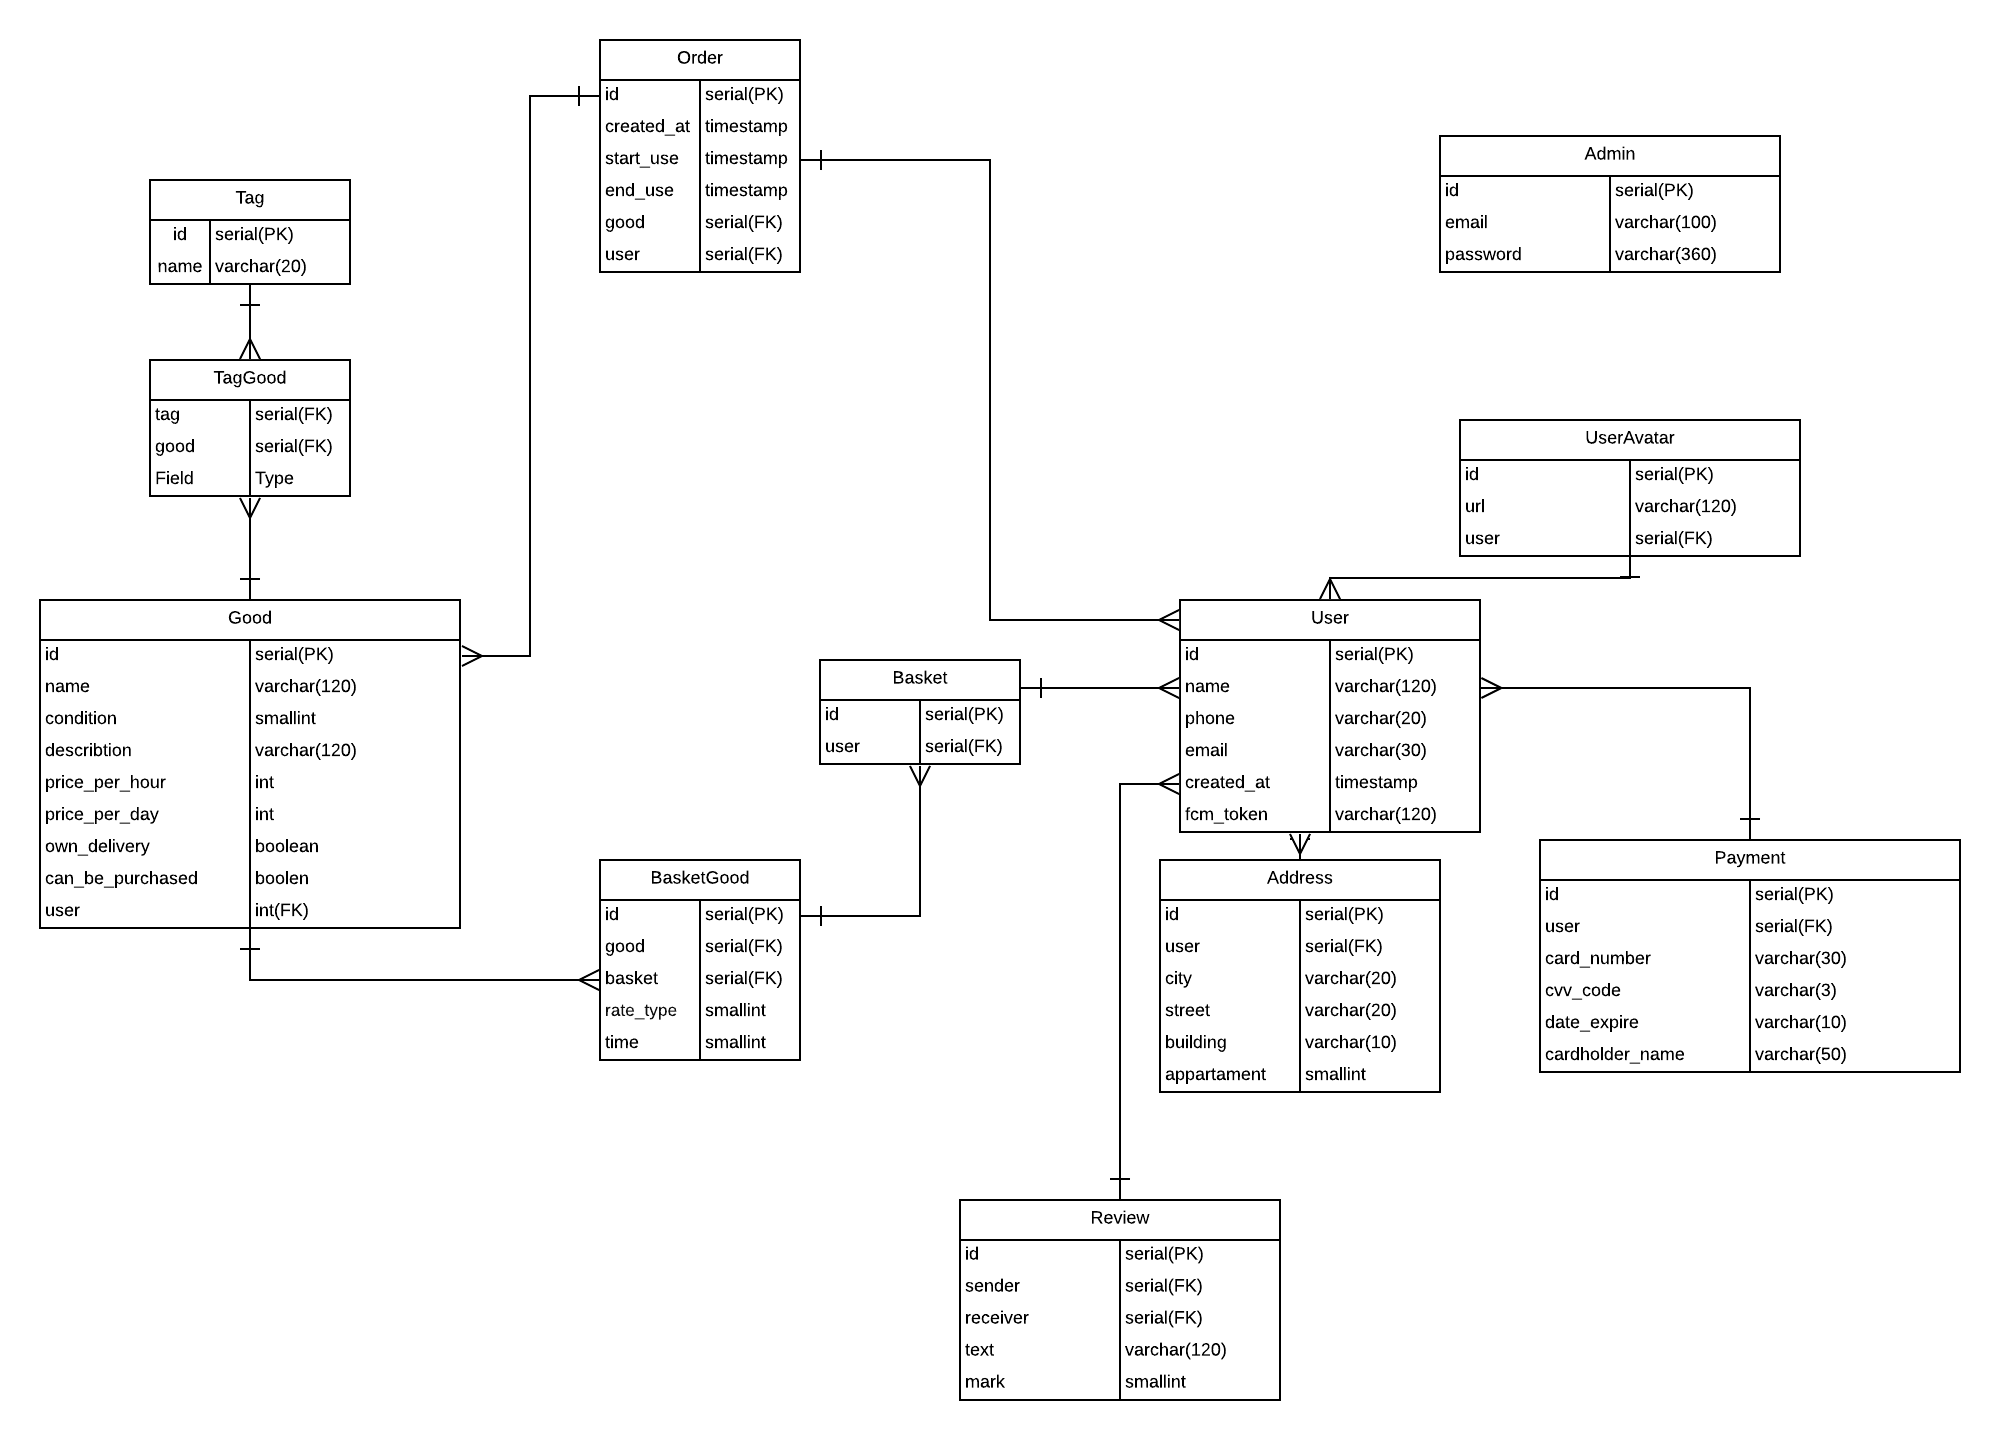
\includegraphics[scale=0.7, angle=90]{erdig.png}
    \caption{ER-диаграмма базы данных}
    \label{db:erdiag}
\end{figure}

\subsubsection{}

При построении баз данных необходимо следовать определённым правилам.
Эти правила получили название нормализации баз данных[14].
Нормализация базы данных является не обязательной, но эти правила существенно упростят работу по составлению запросов и способствуют улучшению масштабируемости.

Преимущества нормализованной базы данных:
\begin{itemize}
    \item Возможность существенно упростить выборки. Получение данных из базы относительно простыми запросами;
    \item Целостность данных. Избежание потерь или искажения информации в базе данных;
    \item Отсутствие избыточности. Данные в таблице не дублируются, что существенно снижает её размер.
\end{itemize}

Результатом проверки спректированной базы данных на соответсвие нормальной форме является таблица \ref{db:normal}.
В описании критериев второй и терьей нормальных форм были опущены критерии о выполнении предыдущих нормальных форм.

\begin{longtable}{ | p{4cm} | p{6cm} | p{4cm} | }
    \caption{Результаты проверки спроектированной базы данных на соответствие номральным формам}
    \label{db:normal}
    \endfirsthead
    \endhead
    \hline
    Нормальная форма  & Критерий соответствия нормально форме & Соответствие нормальной форме \\ \hline
    Первая нормальная форма & Все значения в ячейках должны быть атомарными, то есть содержать ровно одно неделимое значение, а не список из нескольких значений. & Да  \\ \hline
    Вторая нормальная форма & Все поля в таблице должны полностью зависеть от первичного ключа целиком, а не от его части & Да  \\ \hline
    Третья нормальная форма & Значения полей должны зависеть только от первичного ключа, а не от других полей & Да  \\
    \hline
\end{longtable}

В результате была спреоктирована база данных, удовлетворяющая номальной форме.

\subsection{Проектирование архитектуры программного средства}
На основании поставленных задач програмного средства, сформулированных функциональных требований было принято решение выбрать основной для разработки платформу веб-приложений.

Как и у других информационных сервисов Интернет, архитектура Веб основана на принципе клиент-сервер.
На Веб-серверах поддерживаются информационные ресурсы системы, представленные в форме гипертекста или гипермедиа.
Информационные ресурсы Веб-сервера связаны между собой и могут быть связаны с ресурсами других серверов гиперссылками, образуя глобальное информационное гиперпространство.

Ахитектура «клиент-сервер» предоставляет пользователю одно основное преимущество — возможность получить графический пользовательский интерфейс, не модернизируя сервер.

Существует два ключевых момента любой архитектуры:
\begin{itemize}
    \item Число пар операций обмена (запрос, ответ), прежде всего там, где используются медленные и неустойчивые каналы связи;
    \item Строгое разделение задачи управления пользовательским интерфейсом и задачи управления данными.
\end{itemize}

В случае архитектуры «клиент-сервер» обработка данных производится централизованно на сервере.
Клиент посылает запрос к данным, сервер обрабатывает этот запрос и передает клиенту ответ.

Клиентское приложение должно идентифицировать по имени целевой сервер, к которому оно посылает запрос, а поиск физического сервера осуществляется на основании правил разрешения имен.
Эти функции берут на себя серверный и клиентский компоненты СУБД, которые обеспечивают сетевой сервис.
Все вопросы разрешения имен находятся в компетенции настроек этого ПО, а не собственно приложения-клиента.
По сути, приложение-клиент общается непосредственно с клиентским ПО сетевого драйвера СУБД, а не с ядром СУБД.
При этом:
\begin{itemize}
    \item Клиентский и серверный процессы могут находиться как на одной, так и на разных машинах;
    \item Клиентский и серверный процессы могут работать в разном окружении (аппаратное обеспечение, операционная система).
    Архитектура обеспечивает независимость клиентского ПО от серверного ПО СУБД.
    Независимость достигается за счет строго определенного интерфейса обмена, который, в свою очередь, осуществляется посредством посылки сообщений строго определенного формата;
    \item Клиентский процесс не знает, какой сервер в итоге будет обрабатывать его запрос.
    Средства передачи запросов от сервиса к сервису контролируются как СУБД, так и другими серверными процессами (например, запрос был обработан Web-сервером, преобразовавшим его в запрос для монитора транзакций, который обратился непосредственно к СУБД, а передача ответа идет в обратном порядке — в результате клиентский запрос последовательно обработан тремя серверами).
\end{itemize}

Все эти положения, по сути, описывают инкапсуляцию, которая является необходимым условием успешного проектирования в этой архитектуре.
Проектируя любое приложение в архитектуре «клиент-сервер», следует обратить внимание на минимизацию операций обмена между клиентом и сервером.
Вынесение части бизнес-логики на сервер в виде хранимых процедур позволяет снизить количество операций обмена.

Еще одним фактором является количество соединений одного приложения с сервером баз данных.
СУБД на каждое соединение выделяет определенный ресурс.
Если приложение открыло 10 соединений, а работает только одно из них, то СУБД реально резервирует все 10 ресурсов.
Большинство интерактивных приложений характеризуются тем, что более 90\% времени по открытым этими приложениями соединениям не ведется никакой работы.
Для некоторых СУБД большое количество неактивных соединений серьезно снижает эффективность работы сервера.

Основная задача проектирования в архитектуре «клиент-сервер» — реализовать на клиенте качественный прикладной интерфейс (экранные формы и, может быть, небольшое число проверок корректности ввода данных) и осуществить на сервере обработку разделяемых данных.
Наличие тонкого клиента также важно в современных информационных системах.
Большинство серверов баз данных оптимизировано для селективной выборки данных, серверное ПО рассчитано на прием и передачу данных за минимальное время.
Не следует злоупотреблять на разделяемых ресурсах сервера прикладными программами, используемыми клиентами.

Простая клиент-серверная архитектура применяется очень редко и только для очень простых приложений[15].
Для разрабатываемого ПС была выбрана трехуровневая архитектурах[16].

Это архитектурный шаблон, в котором появляется третий участник — хранилище данных.
При использовании этого шаблона, три уровня принято называть слоями:
\begin{enumerate}
    \item Клиентский слой — интерфейс пользователя.
    Это может быть веб-браузер, которому отправляются HTML-страницы, или графическое приложение, написанное с помощью JavaFX.
    Главное, чтобы с его помощью пользователь мог отправлять запросы на сервер и обрабатывать его ответы.
    \item Слой логики — сервер, на котором происходит обработка запросов/ответов.
    Часто его еще называют серверным слоем.
    Также здесь происходят все логические операции: математические расчеты, операции с данными, обращения к другим сервисам или хранилищам данных.
    \item Слой данных — сервер баз данных: к нему обращается сервер.
    В этом слое сохраняется вся необходимая информация, которой пользуется приложение при работе.
\end{enumerate}

Используя такую архитектуру, мы получаем немало плюсов, среди которых:
\begin{itemize}
    \item Возможность построить защиту от SQL-инъекций — это атака на сервер, при которой передается SQL-код, и при выполнении этого кода злоумышленник может воздействовать на нашу базу данных;
    \item Разграничение данных, к которым имеется возможность регулирования пользовательского доступа;
    \item Возможность модифицировать данные перед отправкой клиенту;
    \item Масштабируемость — возможность расширить приложение на несколько серверов, которые будут использовать одну и ту же базу данных;
    \item Меньшие требования к качеству соединения пользователя.
    Формируя ответ на сервере, часто берется из базы данных много различной информации, которая форматируется, и оставляется только то, что нужно пользовтаелю.
    Таким образом сокращается объем информации, который отправляется в качестве ответа клиенту.
\end{itemize}

\subsection{Проектирование клиентской части}
Интерфейс веб-приложения является визуальной частью приложения, с которой взаимодействует пользователь, работая с приложением.
Интерфейс должен быть простым, интуитивно понятным, дружелюбным, визуально приятным в использовании и последовательным. Визуальную составляющую определяет цветовая схема и общая тематика, в которой выполнен дизайн приложения.
Для достижения цели позитивного восприятия интерфейса веб-приложения выбран монотонный, черно-белый дизайн в стиле минимализма.
Данная цветовая гамма и стиль были выбраны для того, чтобы сосредоточить внимание пользователя на товарах.
Верное расположение элементов интерфейса, логические последовательности сценариев веб-приложения и очевидные результаты взаимодействия пользователя с интерфейсом определяет UX(опыт взаимодействия с интерфейсом).

Интерфейс веб-приложения должен включать экраны:
\begin{itemize}
    \item Главная страница с товарами;
    \item Персональная страница пользователя;
    \item Страница управления товарами;
    \item Страница для авторизации в приложении;
\end{itemize}

При выборе инструмента для реализации веб-интерфейса приложения было решено использовать библиотеку React.
Одна из наиболее приятных возможностей React заключается в том, что эта библиотека не принуждает разработчика к строгому соблюдению неких соглашений, касающихся структуры проекта.
Многое в этом плане остаётся на усмотрение программиста.
Они дают разработчикам больше стандартных возможностей.
В этих фреймворках предусмотрены и соглашения, касающиеся структуры проектов, и правила именования файлов и компонентов.

Конечно, можно все приложение описать в одном файле.
Но чем крупнее приложение, тем настойчивей оно требует принятия таких мер, как снижения сложности, и повторное использование компонентов для оптимизации скорости разработки и качества кода.
Каждый уровень абстракции призван облегчить труд разработчика, а терминология предоставить высокий уровень взаимодействия, и разделения обязанностей внутри команды.

Есть множество возможных вариантов организации структуры для проектирования приложения на React и нету одной единственной, которую можно было бы назвать совершенной, потому как каждый приложение преследует свои цели.

Для одной страницы с текстовым резюме все React приложение можно описать в одном файле. Для портальных решений порой не хватает и целого репозитория.

Но существуют проверенные практики.
И начиная разрабатывать приложение на React, стоит хотя бы с ними ознакомится, что спроектировать структуру, а не наращивать поступательно, по мере необходимости, что неизбежно приводит к big ball of mud, в большей или меньшей степени.


\subsubsection{}

\begin{itemize}
    \item Первый тип компонента, с которым создается “Hello, World” или компонент-компонент.
    Презентационные или, как их еще называют, — глупые компоненты. Свое прозвище заслужили тем, что не содержат бизнес логики.
    Концепция умный/глупый компонент описана еще 2015 году.
    С того момента предпринимались попытки и добавить в глупые компоненты бизнес логику, и вкладывать в них контейнеры.
    Но истинная суть неизменна — отделение представления от контролера;
    \item Макеты — это композиция из глупых компонентов.
    Они описывают то, как компоненты расположены на странице (контейнере).
    Макеты не могут содержать бизнес-логики, но должны иметь I/O для ее подключения.
    Макеты полезны при использовании подхода с единым UI Kit , а не представляют из себя монолитную разметку.
    Единственным оправданием существования макетов — это возможность их повторного использования.
    Если разметка используется в приложении только один раз, то эта разметка должна описываться в контейнерах.
    \item Контейнеры — это компоненты, содержащие представление, обернутое в бизнес логику.
    Контейнеры не должны содержать стилей и их представление должно быть составлено из глупых компонентов или макетов.
    Именно контейнеры передаются в prop component Route. В них осуществляется связь между бизнес логикой и представлением.
    Иногда контейнеры могут содержать роутинг. Особенно этого стало актуально с выходом react-route 4.
    Но такой подход сомнителен, поскольку в таком случае возникают сомнения остается ли при этом контейнер контейнером.
    Причинами, оправдывающими существование контейнеров, является их повторное использование и декомпозиция сложных форм.
    Иными словами, создавайте контейнеры, если это обусловлено декомпозицией или их множественным применением — в остальных случаях контейнеры должны описываться в роутах.
    Частым случаем является описание глупых компонентов в контейнерах, в случаях если эти компоненты используются только в данном контейнере.
    Концептуальные границы контейнера очень не устойчивы.
    При достаточно высоком уровне сложности приходит понимание, что контейнер, по сути, превращается в микро-приложение.
    В таком случае стоит задуматься остается ли он при этом контейнером и может стоит подобрать другую категорию компонента.
\end{itemize}

\subsubsection{}

При разработке больших приложений невозможно заранее спланировать устройство всех необходимых моделей.
Более того, по мере того, как размер приложения увеличивается, использование техники внедрения редьюсеров помогает сэкономить большой объём человеко-часов.
Эта техника позволяет разработчикам добавлять в систему новые редьюсеры, не переписывая всё хранилище.

Существуют библиотеки, которые предназначены для создания динамических хранилищ Redux[17].
Однако мне больше нравится механизм внедрения редьюсеров, так как он даёт разработчику определённый уровень гибкости.
Например, этим механизмом можно оснастить существующее приложение и при этом не столкнуться с необходимостью серьёзной реорганизации приложения.
Внедрение редьюсеров — это форма разделения кода.

Существует целый ряд инструментов, которые используются для решения задач маршрутизации в приложениях.
В данном проекте была выбрана библиотека react-router-dom.
Так же были расширены её возможности таким образом, чтобы она могла бы работать с Redux.

Чаще всего маршрутизатор React используют так: корневой компонент заключают в тег BrowserRouter, а дочерние контейнеры оборачивают в метод withRouter() и экспортируют их.
При таком подходе дочерний компонент получает, через механизм props, объект history, содержащий некоторые свойства, специфичные для текущей сессии пользователя.
В этом объекте имеются и некоторые методы, которые могут быть использованы для управления навигацией.

Такой вариант маршрутизации может приводить к возникновению проблем в больших приложениях.
Происходит это из-за того, что в них нет некоего централизованного объекта history.
Кроме того, компоненты, которые не отрисовываются с помощью <Route>, не могут работать с объектом history.

Для решения этой проблемы была использована библиотека connected-react-router, которая позволила наладить маршрутизацию с использованием метода dispatch.
Интеграция в проект этой библиотеки потребует выполнить некоторые модификации.
В частности — нужно будет создать новый редьюсер, предназначенный специально для маршрутов (это вполне очевидно), а так же — добавить в систему некоторые вспомогательные механизмы.

Новой системой маршрутизации, после завершения её настройки, можно пользоваться посредством Redux.
Так, навигация в приложении может быть реализована путём отправки действий.

\subsubsection{}

Redux-saga[18] это библиотека нацеленная делать сайд-эффекты проще и лучше путем работы с сагами.
Саги это дизайн паттерн, который пришел из мира распределенных транзакций, где сага управляет процессами, которые необходимо выполнять транзакционным способом, сохраняя состояние выполнения и компенсируя неудачные процессы.

В контексте Redux, сага реализована как промежуточный слой, который координирует и побуждает асинхронные действия (сайд-эффекты).
Redux-saga делает это с помощью ES6 генераторов.
Генераторы (Generators) это функции которые могут быть остановлены и продолжены, вместо выполнения всех выражений в один проход.

Когда происходит вызов функцию-генератор, сага возвращает объект-итератор.
И с каждым вызовом метода итератора next() тело функции"=генератора будет выполняться до следующего yield выражения и затем останавливаться.
Это делает асинхронный код проще для написания и понимания.

Для координирования логики, которую необходимо реализовать внутри саги, можно использовать вспомогательную функцию takeEvery для создания новой саги для выполнения операции.
Если есть несколько запросов, takeEvery стартует несколько экземпляров саги-рабочего (worker saga).
Иными словами реализует конкурентность(concurrency) для вас.

Надо отметить, что сага-наблюдатель (watcher saga) является другим неявным слоем (layer of indirection), который дает больше гибкости для реализации сложной логики (но это может быть лишним для простых приложений).
Но redux-saga позволяет нам получить объект, который декларирует наше намерение произвести операцию, вместо результата выполнения самой операции.

Вместо вызова асинхронного запроса напрямую, метод call вернет только объект описывающий эту операцию и redux-saga сможет позаботиться о вызове и возвращении результатов в функцию-генератор.
Тоже самое касается и метода put.
Вместо отправления действий (dispatch action) внутри функции"=генератора, put возвращает объект с инструкциями для промежуточного слоя (middleware) — отправить действие.
Эти возвращаемые объекты называются Эффекты.

Работая с эффектами, redux-saga делает саги скорее декларативными, чем императивными.
Декларативное программирование это стиль программирования, который пытается минимизировать или устранить сайд-эффекты, описанием что программа должна делать, вместо описания как она должна это делать.
Преимущество, которое это дает, и о чем говорят большинство людей, то что функцию, которая возвращает простой объект, гораздо проще тестировать, чем функцию, которая делает асинхронный вызов.
